\documentclass[border=0.8ex,svgnames,tikz]{standalone}
\usepackage{amsmath,mathtools}
\usepackage{fontspec}
\setmainfont{Source Serif 4}
\setsansfont{Source Sans 3}
\setmonofont{Source Code Pro}
\usetikzlibrary{positioning,calc}
\def\xcoloruseA{MediumBlue}
\def\xcoloruseB{LimeGreen}
\begin{document}
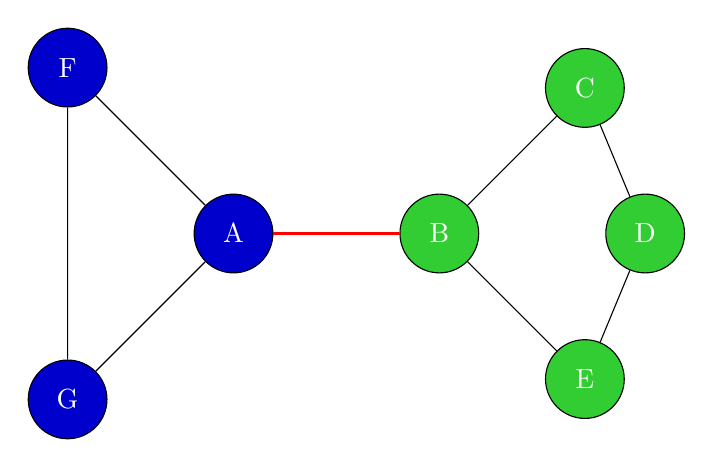
\begin{tikzpicture}[
  node distance=1.6cm,
  every node/.style={draw,circle,minimum size=1cm,text=White},
  every path/.style={draw,>=latex},
  ]
  \coordinate(graph);
  \node[fill=\xcoloruseA,below=of graph] (graphG) {G};
  \node[fill=\xcoloruseA,above=of graph] (graphF) {F};
  \node[fill=\xcoloruseA,right=of graph] (graphA) {A};
  \node[fill=\xcoloruseB,right=of graphA] (graphB) {B};
  \node[fill=\xcoloruseB,below right=of graphB] (graphE) {E};
  \node[fill=\xcoloruseB,above right=of graphB] (graphC) {C};
  \node[fill=\xcoloruseB,right=of graphB] (graphD) {D};
  \path
  (graphA) -- (graphF) -- (graphG) -- (graphA)
  (graphB) -- (graphC) -- (graphD) -- (graphE) -- (graphB);
  \path[Red,thick] (graphA) -- (graphB);
\end{tikzpicture}
\end{document}
